\section{Data}
\label{sec:Data}

\subsection{DDSM}
\label{subsec: Date_DDSM}

Most computer aided diagnosis (in the CADx) 
and detection (CADe) algorithm breast cancer 
was evaluated in a private data set or 
subset unspecified public databases breast 
X-ray imaging.
\cite{Lee2017,Gao2019}
This leads to performance or replicate 
previous results can not be directly comparable 
methods.
\cite{Choukroun2017}
In order to address this major challenge, 
we need to publish digital breast X-ray 
screening database (DDSM) updated and 
standardized version, in order to assess 
breast X-ray photography in the future CADx 
and CADe systems (also sometimes referred to 
as CAD) study.
\cite{Zhu2017}
The CBIS-DDSM (planning DDSM mammography subset), 
including decompressing video data selected by 
trained mammographers curated updated 
segmentation quality, bounding boxes, and 
pathological diagnosis of training data, which 
looks like a modern computer vision data set.
The data set included 753 cases and 891 
calcified mass cases, be able to provide 
analysis and decision support system size of 
data sets in ammography.
As shown in Figure~\ref{fig:figData}

\begin{figure*}[!ht]
    \centering
    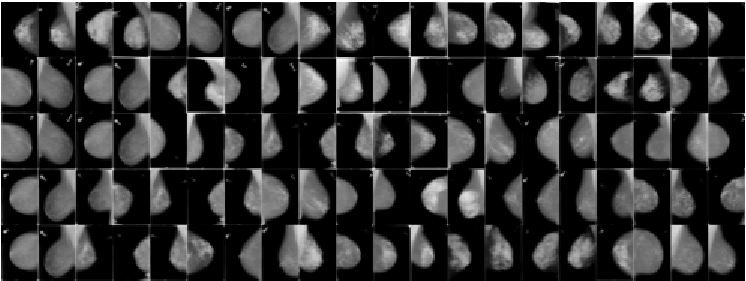
\includegraphics[
        width=1.0\textwidth,
        keepaspectratio
        ]{Data.pdf}
    \caption{Examples in the dataset}
    \label{fig:figData}
\end{figure*}

\subsection{Augmentation}
\label{subsec: Date_Aug}

Compared to the image in the object detection 
field other common data set (e.g., Pascal Voc), 
DDSM data set is relatively small. 
\cite{M.HeathK.BowyerD.Kopans2001}
Since small data sets are prone to reduce the 
model effect, to maintain the representation 
power of model and avoid overfitting in some 
ways, several data augmentation methods are 
employed. 
We don’t augment data with the crop, translate 
or scale operations to avoid changing the 
original label of images.
Instead, we randomly rotate and shear the 
original images between -10$^{\circ}$ and 
10$^{\circ}$ , then flip them horizontally 
or vertically and fill the margin with 
white pixels. 